\documentclass[12pt]{article}
\usepackage{amsmath,amsfonts, epsfig}
\usepackage{booktabs} % for better table formatting
\usepackage[authoryear]{natbib}
\usepackage{array}
\usepackage{multirow}
\usepackage{graphicx}
\usepackage{fancyhdr}
\usepackage{bm}
\pagestyle{fancy}
\lfoot{\texttt{ematm0067.github.io} / \texttt{ematm0044.github.io}}
\lhead{Introduction to AI - 02.3\_regression - Conor}
\rhead{\thepage}
\cfoot{}

\usepackage{tikz}
\usetikzlibrary{positioning}

\usepackage{ifthen}
\newboolean{nopics}
\setboolean{nopics}{true}


\begin{document}

\section*{Linear regression.} 

Recently when doing some research, the details of which are not
relevant here, I measured the relationship between two variables, here
I will just call them $x$ and $y$. The data look like:
\begin{center}
\begin{tabular}{@{}ccccccccc@{}}
\toprule
x & 8 & 9 & 10 & 11 & 12 & 13 & 14 & 15 \\ \midrule
y & 54 & 69 & 75 & 78 & 85 & 102 & 103 & 103 \\ \bottomrule
\end{tabular}
\end{center}
When I plotted these data I was surprised, I had expect it to look
roughly like
\begin{equation}
  y\propto 2^x
\end{equation}
but, as is clear from the scatterplot
\begin{center}
  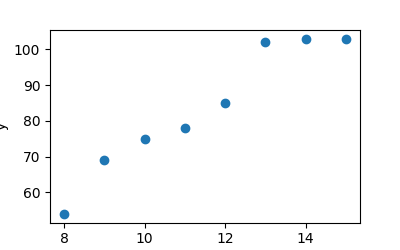
\includegraphics[]{02.3_points.png}
  \end{center}
that it looks a lot more like
\begin{equation}
  y=mx+c
\end{equation}
for some $m$ and $c$. In linear regression we find the values $m$ and
$c$ to give the best line to describe data. This, clearly, raises the
question as to what we mean by best, it also begs the question as to
whether we will know the linear model is a good description or not. We
will answer the first question straight away, the second question is
trickier and we won't consider that here: our intention here is to
find the best line for describing the data under the assumption that
that is a useful thing to do. In practice, data are often described by
a linear model and, if they are, linear models are very easy to use,
so it is often useful to try a linear model first!

The approach we take to deciding what we mean by the `best' line is to
think of the line as a prediction, we think of it as model for the
data, so for each $x$ we have a prediction:
\begin{equation}
  \hat{y}=mx+c
\end{equation}
and this prediction has an error $|\hat{y}-y|$.
\begin{center}
  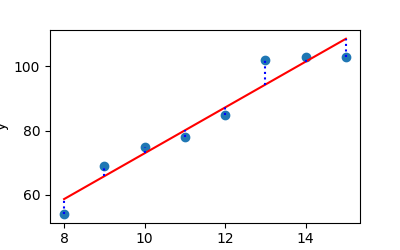
\includegraphics[]{02.3_points_line.png}
  \end{center}
It is typical for models to not make completely accurate predictions,
we imagine that there is some process that is largely responsible for
generating $y$ from $x$ but there is noise: we know that we should
expect the position for an object moving at a constant speed $v$ to be
$vt$, but we also accept that in practice wind or whatever will make
that approximate and our measurement of the position will not be
completely accurate. Nonetheless, we clearly want to minimize the
noise.

However, this does not fully specify what we mean by the error, one
idea would be to sum the individual errors:
\begin{equation}
  \mathcal{E}_1=\frac{1}{n}\sum_i |\hat{y}_i-y|
\end{equation}
where, in the obvious way $\hat{y}_i=mx_i+c$. In fact this would be
very inconvenient because the absolute value can be an awkward object; it has long been common to use the \textsl{root mean square error} instead:
\begin{equation}
  \mathcal{E}_2=\sqrt{\frac{1}{n}\sum_i (\hat{y}_i-y)^2}
\end{equation}
We will see shortly that using the square makes the mathematics of
finding $m$ and $c$ easier, but picking $\mathcal{E}_2$ over
$\mathcal{E}_1$, or indeed over any other error function including
\begin{equation}
  \mathcal{E}_p=\sqrt[p]{\frac{1}{n}\sum_i (\hat{y}_i-y)^2}
\end{equation}
In fact, along with the practical impetus to using $\mathcal{E}_2$,
there is a principled argument based on models of the noise and the
nature of prediction which describes reasonably generic circumstances
where it is the best choice. We will not go into that here.

So, we have decided our task is to pick the $m$ and $c$ that minimize
$\mathcal{E}_2$. In fact, we will consider $\mathcal{E}_2^2$, the
\textsl{mean square error} instead: since the square root is a
monotonically increasing function the values of $m$ and $c$ that
minimize $\mathcal{E}_2^2$ will also minimize
$\mathcal{E}_2$. Substituting in for $\hat{y}_i$ we want to minimize
\begin{equation}
\mathcal{E}_2^2=\frac{1}{n}\sum_i(mx_i+c-y_i)^2
\end{equation}
To minimize we use calculus, a necessary condition for a minimum is that the partial derivatives vanish:
\begin{equation}
\frac{\partial \mathcal{E}_2^2}{\partial m}=\frac{\partial \mathcal{E}_2^2}{\partial c}=0
\end{equation}
Obviously this does not rule out the possibility of a saddlepoint or
maximum, but in this example we are fortunate, looking at the form of
$\mathcal{E}_2^2$ is should be clear that any stationary point is a
minimum, this is easy enough to prove with second order derivatives,
but we won't go into that here.

The derivatives are easy enough using the chain rule, to remind you,
if $f(x)=d(u(x))$ then the rate of change of $f$ with $x$ is the
multiple of how $f$ changes with $u$ and how $u$ changes with $x$:
\begin{equation}
\frac{df}{dx}=\frac{df}{du}\frac{du}{dx}
\end{equation}
The chain rule is easy to remember because it sort of makes sense but
it is also incredibly powerful, allowing any calculation you can
perform to be differentiated. As an aside this is the essence of
\texttt {autograd}, the automatic differentiation routines that make
modern machine learning possible. 

In the case here let $u_i=mx_i+c-y_i$ so
\begin{equation}
\mathcal{E}_2^2=\frac{1}{n}\sum_iu_i^2
\end{equation}
and
\begin{equation}
\frac{\partial \mathcal{E}_2^2}{\partial c}=\sum_i\frac{\partial u_i^2}{\partial c}=\sum_i\frac{d u_i^2}{du_i}\frac{\partial u_i}{\partial c}=2\sum_i u_i
\end{equation}
since the derivative of $u_i$ with respect to $c$ is just one. Hence,
one of the two conditions is
\begin{equation}
0=\sum_i u_i = m\frac{1}{n}\sum_i x_i + c\frac{1}{n}\sum_i 1-\frac{1}{n}\sum_i y_i
\end{equation}
and using a bar for the sample mean of a quantity:
\begin{equation}
\bar{z}=\frac{1}{n}\sum_i z_i
\end{equation}
we get
\begin{equation}
m\bar{x}+c=\bar{y}
\end{equation}
We can also work out the other derivative:
\begin{equation}
\frac{\partial \mathcal{E}_2^2}{\partial m}=\frac{1}{n}\sum_i x_iu_i
\end{equation}
and setting this to zero gives:
\begin{equation}
 m\langle x_i^2\rangle_i +c\bar{x}=\langle x_iy_i\rangle_i
\end{equation}
where the $\langle\ldots\rangle_i$ is used for more complicated sample
means, that is I could've written $\overline{xy}$ instead of $\langle
x_iy_i\rangle_i$. In any case we can now solve for $m$ and $c$, we get
\begin{equation}
m=\frac{\langle (x_i-\bar{x})(y_i-\bar{y})\rangle_i}{\langle (x_i-\bar{x})^2\rangle_i}
\end{equation}
and
\begin{equation}
c=\bar{y}-m\bar{x}
\end{equation}
Thus $m$ depends on the sample average of the auto- and cross-correlation.

Lets do the example above! There are eight samples with
\begin{equation}
\bar{x}=\frac{8+9+10+11+12+13+14+15}{8}=11.5
\end{equation}
and
\begin{equation}
\bar{y}=\frac{54 + 69 + 75 + 78 + 85 + 102 + 103 + 103}{8}=83.625
\end{equation}
Similarly
\begin{equation}
\langle (x_i-\bar{x})(y_i-\bar{y})\rangle_i=\frac{1}{8}\sum_i(x_i-11.5)(y_i-83.625)=\approx 37.56
\end{equation}
and
\begin{equation}
\langle (x_i-\bar{x})^2\rangle_i=\frac{1}{8}\sum_i(x_i-11.5)^2=\approx 5.25
\end{equation}
giving $m=7.1548$ and $c=1.3452$.

\subsection*{More dimensions}

Many of you will recognize this algorithm as the ordinary
\textsl{least squares approximation}, which is what it is; we call it
by this other name \textsl{linear regression} because we want first to
link it to other types of regression; by regression we mean fitting a model of the data:
\begin{equation}
  \hat{y}=f(x;\theta)
\end{equation}
for some function $f(x;\theta)$, where $\theta$ are parameters used to
specify the function precisely, in fitting the data are used to fix
the values of the parameters $\theta$. In linear regression the model
is linear $\hat{y}=mx+c$ and the parameters are
$\theta=\{m,c\}$. Linear regression is the most straight-forward
non-trivial model, we will see other examples later.

The second reason to refer to linear regression is that ordinary least
squares usually just refers to the one-dimesional problem, where $x$
and $y$ are just numbers. Obviously we are often interested in
outcomes that have more than one cause or where the outcome is
described by more than one number, that is, where we have vectors,
$\mathbf{x}$ or, or possibly and, $\mathbf{y}$. There is a notational
problem that bedevils our subject, which is to avoid confusing
`trials' and `components'. In the example above $x$ is just a scalar,
in the experiment we had a set of different measured values we called
$\{x_1,x_2,\ldots,x_n\}$, in other words the index in $x_i$ is a
trial or sample index, corresponding to different measured values. If
$\mathbf{x}$ is a vector then we might want to write
\begin{equation}
  \mathbf{x}=(x_1,x_2,\ldots,x_d)
\end{equation}
where $\mathbf{x}$ is a $d$-dimensional vector. Now if we have trials
we might write that them as
$\{\mathbf{x}_1,\mathbf{x}_2,\ldots,\mathbf{x}_n\}$ with, for example
\begin{equation}
  \mathbf{x}_1=(x_{11},x_{21},\ldots,x_{d1})
\end{equation}
and so on. However there is largely a lot of sloppiness across the
field. Another approach is to use a matrix, so $X$ is the matrix
\begin{equation}
  X=[x_{ij}]
\end{equation}
where the first index is the component index and the second the trial
index. This is certainly convenient when it comes to writing computer
code, but mathematically it is ugly since it combines in a matrix two
very different types of index and because you often find yourself
doing a lot of messing to distinguish row and column vectors, or you
ignore that distinction and people who are obsessed with that
distinction get confused. In short, always try to be carefull with
your own notation but don't trust anyone elses.

However, the mathematics is not much worse for multidimensional linear
regression; most of the difficulty is a problem with keeping track of
what you are doing. For simplicity we will look at the case with $y$ a scalar, then we have something like
\begin{equation}
  \hat{y}=\beta_0+\beta_1x_1+\beta_2x_2+\ldots+\beta_dx_d
\end{equation}
or in vector notation
\begin{equation}
  \hat{y}=\beta_0+\boldsymbol{\beta}\cdot\mathbf{x}=\beta_0+\boldsymbol{\beta}^T\mathbf{x}
\end{equation}
where
\begin{equation}
  \boldsymbol{\beta}=(\beta_1,\beta_2,\ldots,\beta_d)
\end{equation}
For some reason it is very common to use beta for regression
coefficients. Now, if we use
\begin{equation}
  \hat{\textbf{y}}=(\hat{y}_1,\hat{y}_2,\ldots,\hat{y}_n)
\end{equation}
to correspond to estimates for different trials, we can write
\begin{equation}
  \hat{\textbf{y}}^T=\beta_0\mathbf{1}+\boldsymbol{\beta}^TX
\end{equation}
where $\mathbf{1}$ is a vector of ones. As an aside, it is a common
trick to add an extra `zero-th' value to the vector $\mathbf{x}$ so
that it becomes
\begin{equation}
  \mathbf{x}=(1,x_1,x_2,\ldots,x_d)
\end{equation}
and we can write the regression model as
\begin{equation}
  \hat{\textbf{y}}^T=\boldsymbol{\beta}^TX
\end{equation}
where
$\boldsymbol{\beta}=(\beta_0,\beta_1,\beta_2,\ldots,\beta_d)$. Either
way, we can do the same sort of calculation as before to find an
equation for all the $\beta$s; we won't go through the details here,
but it really follows the same strategy as before.

As one final note, regression models often need to be
regularized. What that means is that there is not really enough data
and outliers can have a disproportionate effect on the result. A
regularization approach adds some assumptions about the behaviour of
$y$, some sort of assumption about its variance for example. The most
common regularised regression methods are \textsl{ridge regression} or
\textsl{lasso regression}. We won't discuss these here, but you are
likely to encounter them in data science.

\subsection*{Gradient flow}

To go back to the example above, we wanted to find the best $m$ and $c$ by finding the values that minimized the error:
\begin{equation}
\mathcal{E}_2^2=\frac{1}{n}\sum_i(mx_i+c-y_i)^2
\end{equation}  
Here is what that function looks like, using a contour plot, the
curves mark equal values of the error across the $mc$-plane, just as
contours on a map mark places that are at the same height:
\begin{center}
  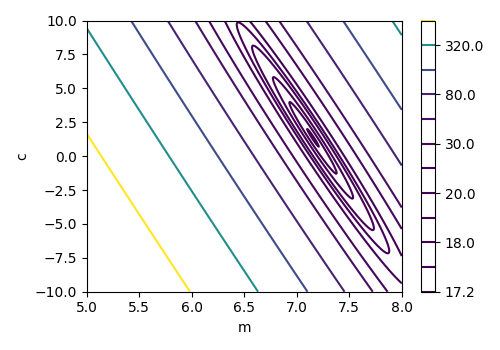
\includegraphics[]{02.3_contour.png}
  \end{center}
Note that for illustrative purposes the contours are not equally
spaced. The mathematics we did brought us to the very bottom of the
landscape, in the middle of the smallest oval.

Now we are fortunate in this case to be able to solve explicitely for
the minimum of $\mathcal{E}_2^2$; we call this having an
\textsl{analytic} or a \textsl{closed form} solution and it is unusual
in this context. Typically, for more complicated models, we can't find
a solution exactly and so we resort to approximate methods. One such
method is `gradient flow'; basically, if we imagine the error as a
landscape, gradient flow says we should try to go downhill.

We can do that because we actually know what direction is downhill, or
rather, we know the direction of uphill. It is the gradient, the
vector made out of partial derivatives. From now on to make things tidier we are going to drop the two twos on the error function and write $\mathcal{E}$ rather than $\mathcal{E}_2^2$. Now the gradient is
\begin{equation}
  \boldsymbol{\nabla} \mathcal{E}=\left(\frac{\partial\mathcal{E}}{\partial m},\frac{\partial\mathcal{E}}{\partial c}\right)
\end{equation}
This vector points straight up the hill so the idea is to take a little step down the hill:
\begin{align}
  m&\leftarrow m-\eta\frac{\partial\mathcal{E}}{\partial m}\\
  c&\leftarrow c-\eta\frac{\partial\mathcal{E}}{\partial c}
\end{align}
where $\eta$ is a small number, called the learning rate, to make sure
that it is only a little step, the greek letter `eta' is often used
for small values. Since the gradient is changing from place to place
so taking too long a step might mean you go too far and end up going
up hill instead of down, like a giant striding over valleys. Of
course, gradient flow has to start somewhere, the idea is to guess a
good starting place and then take steps down the hill in the hope of
getting to the bottom, that is the minimum of the error function.

The error function we have been using, from some real data, is very oblong-ish and it is tricky to use it to illustrate gradient flow. As such for drawing some pictures we will use a simpler error:
\begin{equation}
  \mathcal{E}=(m-2)^2+(1.5c-3)^2
\end{equation}
The contours are
\begin{center}
  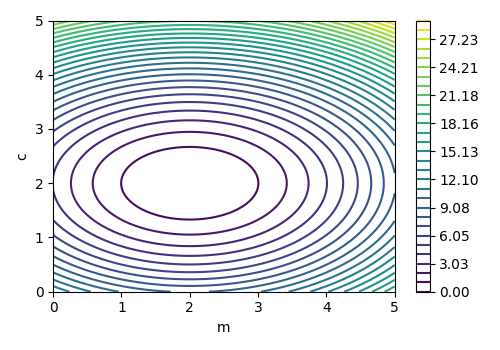
\includegraphics[]{02.3_simple_contour.png}
  \end{center}
Now the gradient is easy to calculate:
\begin{equation}
  \boldsymbol{\nabla} \mathcal{E}=\left(2(m-2),3(1.5c-3)\right)
\end{equation}
and we can plot the gradient descent with $\eta=0.1$ and starting point $(0,0)$
\begin{center}
  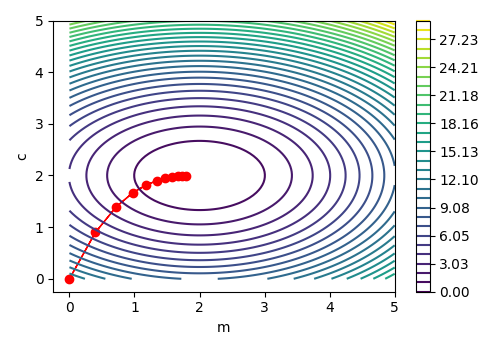
\includegraphics[]{02.3_gradient.png}
  \end{center}
If $\eta=0.43$ the gradient descent begins to jump backwards and
forwards across the minimum, bigger values lead to even more
disasterously erratic behaviour.

In short, one convenient aspect of linear regression is that it is
straight-forward to solve for the minimum by finding the point where
the gradient is zero. As an illustration of a more general approach we
consider gradient descent, this is what we call a numerical approach,
one that produces a number answer rather than a general formula. It
works by calculating the gradient of the error function and then using
that to repeatedly update the parameters in a way that, hopefully,
reduces the error. Obviously there are a few hazards, obviously
picking $\eta$ is one, too big and it can lead to inefficient or
erratic behaviour, too small and the algorithm wastes a lot of time
moving in tiny steps and not going anywhere much. The problem is for
some problems we have little idea what scale corresponds to a large or
small value. A second problem is that gradient flow does not
distinguish between local and global minima, if there are lots of
local minima the algorithm won't find the global minimum.

In fact, gradient flow, in some form or another, is at the center of a
lot of modern data science: as alluded to above, the use of the chain
rule across all the small steps that make up any computer calculation
allow \texttt{autograd} commands to calculate gradients. Similarly
there are approaches to the other problems mentioned that work, maybe
not all the time, but more than you might've guess: stochastic
gradient flow, which effectively introduces noise into estimates by
only using partial data, appears to help with avoiding local minima,
for example, and newer algorithms, like Adam, which are based on
gradient flow but have adaptive behaviour, rely less on a good choice
of learning rate.

\section*{Summary}
In linear regression we assume the data come from a noisy version of a
linear process and we seek to model that process. It turns out there
is an analytic formula for the model parameters. This generalizes to
linear models that have lots of inputs and lots of predictions. The
error associated with the model can be minimimized by gradient flow,
since this is a solved problem it seems weird to do it approximately,
however numerical approaches like gradient descent works in other
cases where there is no analytic solution. We see how gradient on our
simple example.
\end{document}

